\chapter[Introdução]{Introdução}
\label{chap:introducao}

\section{Contexto}
\label{sec:introducao-contexto}

A abordagem territorial no desenvolvimento rural brasileiro consolidou-se, nas
últimas décadas, como estratégia de descentralização e fortalecimento da
agricultura familiar. Após um período de descontinuidade, a política territorial
atravessa uma fase de retomada sob coordenação da Secretaria de Governança
Fundiária, Desenvolvimento Territorial e Socioambiental (SFDT), vinculada ao
Ministério do Desenvolvimento Agrário e Agricultura Familiar (MDA). Para
viabilizar essa retomada, o MDA firmou Termo de Execução Descentralizada (TED)
com o Centro de Gestão e Inovação da Agricultura Familiar (Cegafi), plataforma
tecnológica do Parque Científico e Tecnológico da Universidade de Brasília, no
âmbito do projeto Monitora Territórios.

O projeto Monitora Territórios, executado nesse âmbito, atua na organização da
gestão de 174 territórios e na criação de 26 novos colegiados, e tem no Sistema
de Informações Territoriais (SIT) o repositório oficial dos dados de
acompanhamento. Sua atuação distribui-se em frentes temáticas distintas: o
fortalecimento institucional dos colegiados territoriais; o planejamento
territorial, conduzido por meio de oficinas participativas e de ferramentas
digitais de geoprocessamento; a agroecologia e o abastecimento, que aproximam a
agricultura familiar de mercados digitais e de políticas como o PAA e o PNAE; a
ampliação do acesso ao crédito rural e à assistência técnica nos territórios
vinculados ao PAS Nordeste; o desenvolvimento multidimensional, que incorpora
cultura, gênero, saúde e turismo rural; e a compensação das emissões de carbono
associadas às próprias atividades do projeto \cite{cegafi2026}.

Essa amplitude temática tem consequência direta sobre o problema aqui tratado.
Cada frente carrega o seu próprio conjunto de normativos, manuais e roteiros
operacionais --- o PAA e o PNAE possuem regras próprias, assim como o crédito
rural, os procedimentos de geoprocessamento e o protocolo das oficinas
territoriais. O acervo que orienta a execução não é, portanto, um documento
único, e sim uma coleção heterogênea, mantida por instâncias distintas e
atualizada em ritmos distintos. A execução do projeto é intensiva em
documentação, e essa característica se manifesta em duas frentes operacionais.

A primeira frente é a consulta. Executar corretamente cada etapa das atividades
previstas exige recorrer a um acervo composto por manuais, protocolos, roteiros
metodológicos, portarias e normativos. Esses documentos são extensos,
encontram-se descentralizados entre repositórios e canais distintos, e passam
por revisões periódicas que geram versões concorrentes. Localizar uma informação
específica exige percorrer o material manualmente, e não há canal formal previsto
para o esclarecimento de dúvidas operacionais --- de modo que a mesma pergunta
é respondida de formas diferentes, por pessoas diferentes, sem que a resposta
fique registrada em qualquer lugar.

A segunda frente é a análise. A cada ciclo mensal, a equipe do Cegafi recebe da
ordem de 174 relatórios, cada um acompanhado de anexos, comprovantes e registros
em mídia, além de campos abertos preenchidos em texto livre. A conferência desse
material é feita relatório a relatório, sem recursos de agregação ou
consolidação automática, o que faz com que inconsistências só se tornem visíveis
ao final do processo --- quando a correção já custa um novo ciclo de idas e
vindas.

O resultado combinado é a demora. Não se trata de um volume de dados grande em
termos computacionais: 179 registros por mês é uma quantidade modesta para
qualquer sistema de informação. O volume é excessivo para leitura e tratamento
humanos, que é exatamente como o processo funciona hoje. A
Figura~\ref{fig:causa-efeito-demora} sistematiza as causas identificadas.

\begin{figure}[htb]
	\centering
	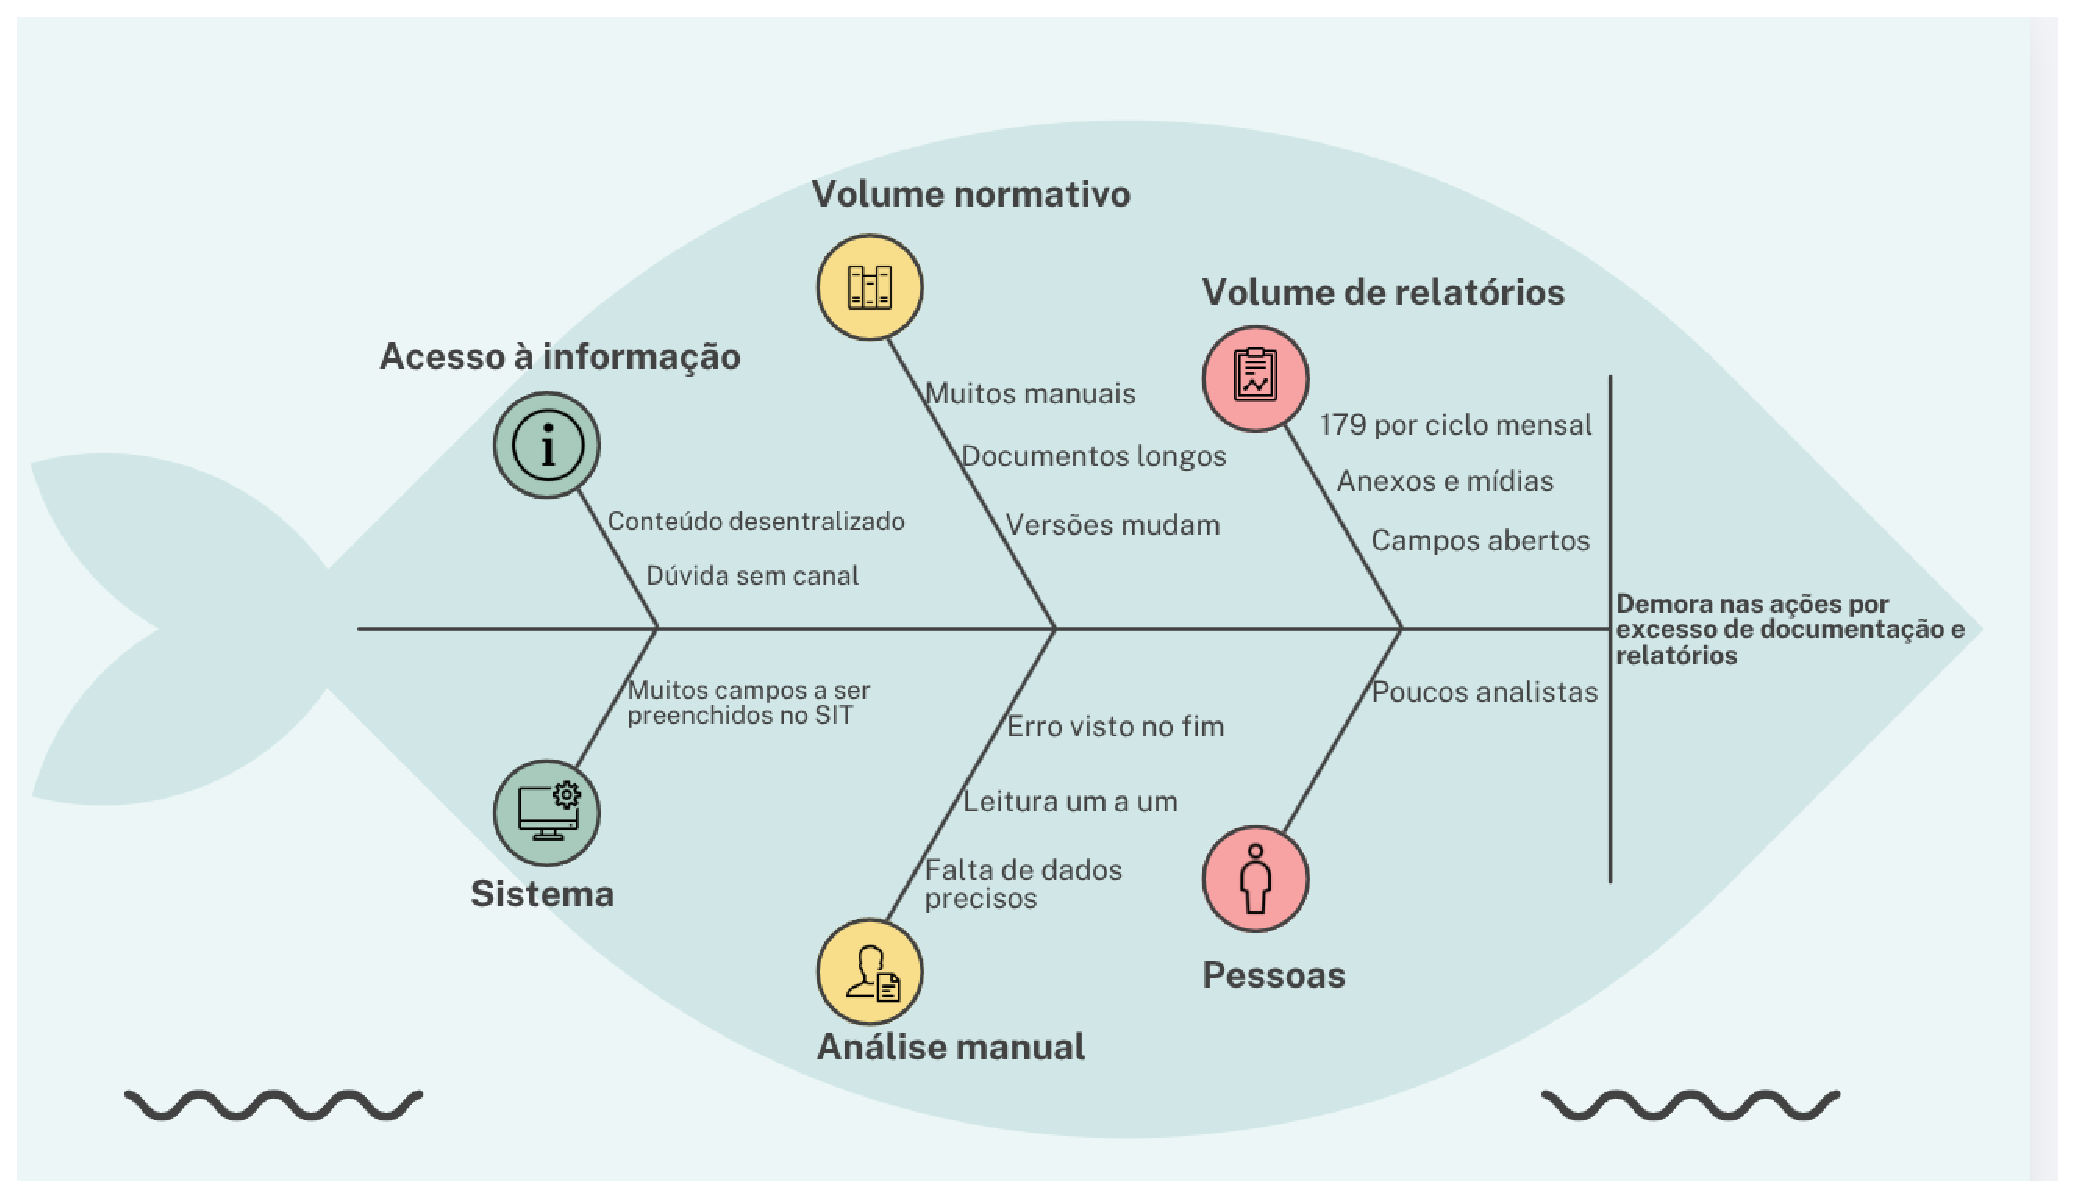
\includegraphics[keepaspectratio=true,width=\textwidth]{figuras/diagrama-causa-efeito-demora.eps}
	\caption{Diagrama de causa e efeito da demora nas ações do projeto}
	\label{fig:causa-efeito-demora}
\end{figure}

É nesse cenário que se coloca a oportunidade explorada por este trabalho.
Avanços recentes em modelos de linguagem de grande porte, combinados a
arquiteturas de \textit{Retrieval-Augmented Generation} --- que ancoram as
respostas do modelo em documentos recuperados de uma base controlada, em vez de
depender apenas de seu conhecimento paramétrico \cite{lewis2020} ---, tornaram
viável consultar acervos documentais extensos em linguagem natural, com
rastreabilidade da fonte, e sintetizar grandes conjuntos de texto não
estruturado. As mesmas técnicas endereçam, portanto, as duas frentes: a consulta
ao acervo normativo e a análise consolidada dos relatórios.

\FloatBarrier
\section{Justificativa}
\label{sec:introducao-justificativa}

A relevância do trabalho está na natureza do gargalo. Ele não decorre de falha
de projeto do processo nem de excesso de exigência documental: os itens
solicitados são requisitos de prestação de contas de recurso público e não podem
simplesmente ser suprimidos. O gargalo decorre da forma como esse material é
acessado e lido, que permanece manual em ambas as pontas.

Essa distinção importa porque delimita o tipo de solução cabível. Não se propõe
reduzir o que se coleta, e sim alterar o modo como o acervo é consultado e como
os relatórios são consolidados. É uma intervenção de engenharia de software
sobre um processo de informação, não uma reformulação da política pública.

Do ponto de vista dos beneficiários, o trabalho interessa a três públicos. Aos
profissionais que atuam nos territórios, por reduzir o tempo gasto localizando
informação normativa e por padronizar as respostas às dúvidas recorrentes. À
equipe de análise do Cegafi, por reduzir o esforço de consolidação e permitir que
inconsistências sejam percebidas antes do fechamento do ciclo. À coordenação do
projeto, por encurtar o intervalo entre a execução das atividades e a
disponibilidade da informação consolidada.

Há ainda um benefício indireto relevante. O registro sistemático das perguntas
dirigidas ao agente produz evidência empírica sobre quais pontos da documentação
oficial são efetivamente ambíguos --- informação que hoje não existe em lugar
nenhum e que pode ser devolvida ao projeto como insumo para revisão dos próprios
manuais.

Do ponto de vista acadêmico, a literatura sobre \textit{Retrieval-Augmented
Generation} concentra-se em avaliação com \textit{benchmarks} de domínio geral
e em ambientes controlados. São escassos os estudos que reportem o desenho, a
implantação e a avaliação desses sistemas sobre acervos normativos e dados
operacionais de política pública brasileira, com usuários reais e em condições
de campo.

\section{Problema}
\label{sec:introducao-problema}

O problema que este trabalho se propõe a investigar é:

\begin{quote}
\textbf{Em que medida sistemas apoiados em modelos de linguagem de grande porte
podem reduzir o tempo despendido na consulta ao acervo normativo e na análise
consolidada dos relatórios do projeto Monitora Territórios, sem perda de
fidelidade às fontes nem de exatidão nos valores reportados?}
\end{quote}

A questão desdobra-se em três dimensões de investigação:

\begin{itemize}
	\item \textbf{Redução de tempo} --- o uso das soluções encurta, de forma
	verificável, o tempo de localização de informação normativa e o tempo de
	consolidação dos relatórios?

	\item \textbf{Fidelidade às fontes} --- as respostas do agente estão
	ancoradas nos documentos recuperados, sem afirmar o que a fonte não sustenta?

	\item \textbf{Exatidão das análises} --- os valores agregados produzidos
	correspondem aos dados reais, condição indispensável para uso em prestação de
	contas?
\end{itemize}

\section{Objetivos}
\label{sec:introducao-objetivos}

\subsection{Objetivo Geral}

Desenvolver e avaliar dois artefatos apoiados em modelos de linguagem de grande
porte --- um agente conversacional para consulta ao acervo normativo e um
sistema de apoio à análise consolidada dos relatórios registrados no SIT --- com
vistas a reduzir o tempo despendido nessas duas atividades no âmbito do projeto
Monitora Territórios.

\subsection{Objetivos Específicos}

\begin{itemize}
	\item \textbf{(OE1)} Caracterizar o acervo normativo e o processo atual de
	análise dos relatórios, identificando as dúvidas e os erros recorrentes.

	\item \textbf{(OE2)} Constituir as bases de conhecimento dos artefatos e os
	conjuntos de avaliação correspondentes, com respostas de referência validadas
	por especialistas.

	\item \textbf{(OE3)} Projetar e implementar o agente conversacional de
	consulta, acessível por canal de baixo atrito para os usuários em campo.

	\item \textbf{(OE4)} Projetar e implementar o sistema de apoio à análise
	consolidada dos relatórios, sob arquitetura que separa consulta determinística
	de síntese textual.

	\item \textbf{(OE5)} Avaliar a qualidade das respostas do agente e a exatidão
	das análises produzidas por meio de experimentos controlados.

	\item \textbf{(OE6)} Avaliar, em uso real, a redução de tempo obtida e a
	usabilidade das soluções junto aos seus respectivos públicos.
\end{itemize}

\section{Metodologia (Resumida)}
\label{sec:introducao-metodologia}

O trabalho adota abordagem mista, enquadrada como \textit{Design Science
Research} (DSR), metodologia adequada a pesquisas cujo resultado central é um
artefato tecnológico projetado para resolver um problema de classe identificada
em contexto real \cite{hevner2004,wieringa2014}. O ciclo de identificação do
problema, projeto do artefato, demonstração e avaliação organiza as fases
descritas a seguir e é detalhado no Capítulo 3.

A Fase 1 caracteriza o problema em campo, por meio do inventário do acervo
documental, de entrevistas com a equipe de análise do Cegafi e do mapeamento da
estrutura dos relatórios registrados no SIT. A Fase 2 prepara os insumos:
tratamento e segmentação do acervo, construção do conjunto de perguntas de
referência e definição das regras de cálculo dos indicadores de consolidação.

A Fase 3 projeta e implementa os artefatos. O agente conversacional é construído
com o núcleo de recuperação exposto por interface própria e o canal implementado
como adaptador, decisão que preserva a possibilidade de avaliação mesmo diante
de restrições externas de acesso. O sistema de análise adota arquitetura
híbrida: os campos estruturados são consultados de forma determinística, cabendo
ao modelo de linguagem a síntese dos campos abertos e a redação da narrativa,
jamais a execução de contagens ou agregações. Essa separação responde a uma
limitação conhecida dos modelos de linguagem em operações de cálculo e é
condição para que os números reportados sejam auditáveis.

A Fase 4 avalia os artefatos. A avaliação controlada afere métricas de
recuperação e de fidelidade às fontes para o agente, e a exatidão das agregações
contra verdade de referência calculada para o sistema de análise. A avaliação
em uso real compara os tempos observados com uma linha de base estabelecida a
partir de ciclos anteriores e aplica instrumentos de usabilidade junto aos
participantes.

A Tabela~\ref{tab:alinhamento-objetivos-atividades} apresenta o alinhamento
entre os objetivos específicos e as atividades a serem executadas. O
detalhamento dessas informações encontra-se no Capítulo 3.

{\small
\renewcommand{\arraystretch}{1.15}
\begin{longtable}{|p{0.31\textwidth}|p{0.61\textwidth}|}
\caption{Alinhamento entre objetivos específicos e atividades}
\label{tab:alinhamento-objetivos-atividades} \\
\hline
\textbf{Objetivo Específico (OE)} & \textbf{Atividades} \\
\hline
\endfirsthead

\caption[]{Alinhamento entre objetivos específicos e atividades (continuação)} \\
\hline
\textbf{Objetivo Específico (OE)} & \textbf{Atividades} \\
\hline
\endhead

\hline
\multicolumn{2}{r}{\textit{Continua na próxima página}} \\
\endfoot

\hline
\endlastfoot

\textbf{(OE1)} Caracterizar o acervo normativo e o processo atual de análise
dos relatórios.
& \textbf{(A1)} Inventariar os manuais, protocolos, roteiros e normativos que
orientam a execução do projeto, registrando volume, formato e estado de
atualização.

\smallskip
\textbf{(A2)} Realizar entrevistas semiestruturadas com a equipe de análise do
Cegafi para levantar os erros e as dúvidas mais frequentes.

\smallskip
\textbf{(A3)} Mapear a estrutura dos relatórios registrados no SIT,
distinguindo campos estruturados de campos abertos e anexos. \\
\hline

\textbf{(OE2)} Constituir as bases de conhecimento e os conjuntos de avaliação.
& \textbf{(A4)} Tratar e segmentar o acervo documental, incluindo extração de
texto de documentos não pesquisáveis.

\smallskip
\textbf{(A5)} Elaborar conjunto de perguntas com respostas de referência
validadas por especialistas do Cegafi.

\smallskip
\textbf{(A6)} Definir os indicadores de consolidação exigidos pela prestação de
contas e suas regras de cálculo. \\
\hline

\textbf{(OE3)} Projetar e implementar o agente conversacional de consulta.
& \textbf{(A7)} Projetar a arquitetura da solução, com separação entre o núcleo
de recuperação e o adaptador de canal.

\smallskip
\textbf{(A8)} Implementar o pipeline de indexação, recuperação e geração de
respostas com citação da fonte consultada.

\smallskip
\textbf{(A9)} Implementar o adaptador de canal para WhatsApp, incluindo
tratamento de áudio e registro das interações. \\
\hline

\textbf{(OE4)} Projetar e implementar o sistema de apoio à análise consolidada
dos relatórios.
& \textbf{(A10)} Implementar a camada de consulta determinística sobre os campos
estruturados dos relatórios.

\smallskip
\textbf{(A11)} Implementar a sumarização temática dos campos abertos por
estratégia de mapeamento e consolidação.

\smallskip
\textbf{(A12)} Implementar a geração dos artefatos consolidados que subsidiam a
prestação de contas. \\
\hline

\textbf{(OE5)} Avaliar a qualidade das respostas e a exatidão das análises.
& \textbf{(A13)} Executar a avaliação \textit{offline} do agente, aferindo
métricas de recuperação e de fidelidade às fontes.

\smallskip
\textbf{(A14)} Aferir a exatidão das agregações produzidas contra verdade de
referência calculada sobre os dados.

\smallskip
\textbf{(A15)} Analisar os casos de falha e ajustar os parâmetros das soluções.
\\
\hline

\textbf{(OE6)} Avaliar a redução de tempo e a usabilidade em uso real.
& \textbf{(A16)} Estabelecer a linha de base de tempo de consulta e de tempo de
análise a partir de ciclos anteriores.

\smallskip
\textbf{(A17)} Conduzir piloto com os usuários das duas frentes durante ao menos
um ciclo mensal.

\smallskip
\textbf{(A18)} Comparar os tempos observados com a linha de base e aplicar
instrumentos de usabilidade e utilidade percebida. \\
\end{longtable}
}

\section{Estrutura do Trabalho}
\label{sec:introducao-estrutura}

O restante do documento organiza-se da seguinte forma. O Capítulo 2 apresenta a
fundamentação teórica, abordando modelos de linguagem de grande porte,
arquiteturas de \textit{Retrieval-Augmented Generation}, estratégias de
sumarização de grandes volumes textuais, métricas de avaliação desses sistemas e
trabalhos correlatos aplicados à administração pública. O Capítulo 3 detalha a
metodologia, o design da pesquisa e os métodos empregados em cada fase. O
Capítulo 4 relata a execução das atividades e os resultados obtidos. O Capítulo
5 analisa e discute esses resultados à luz da literatura e das limitações do
estudo. O Capítulo 6 apresenta as considerações finais e as possibilidades de
trabalhos futuros.
